\documentclass[12pt]{article}

\usepackage[utf8]{inputenc}
\usepackage[brazil]{babel}
\usepackage[a4paper,left=3cm, right=2cm,top=2.5cm, bottom=2.5cm]{geometry}
\usepackage{amsmath}
\usepackage{graphicx}
\usepackage{float}
\usepackage{multirow}
\usepackage{authblk}
\usepackage{fancyhdr}
\usepackage{xcolor}

\title{\textbf{ENG1456 - Redes Neurais - Trabalho 1 Classificação}}
\author{\textbf{Aluno: Matheus Carneiro Nogueira}}
\affil{}
\author{\textbf{Professora: Marley Velasco}}
\affil{}
\pagestyle{fancy}
\fancyhf{}
\lhead{{\small \textcolor{gray}{PUC-Rio ENG1456}}}
\renewcommand{\headrulewidth}{0pt}
\date{}
\renewcommand{\footrulewidth}{0pt}
\fancyfoot[C]{\thepage}

\begin{document}
	\maketitle
	\tableofcontents
	
\begin{abstract}
	Este documento consiste no relatório do trabalho 1 do módulo de Redes Neurais da disciplina ENG1456 da PUC-Rio. Nele será explicada a implementação de modelos de Redes Neurais MLP para a clafficicação do dataset Ionosphere, disponibilizado pela professora da disciplina e disponível em \cite{Dataset}. A seções do relatório são definidas de acordo com as perguntas principais que constam no arquivo Guia de Atividades.
\end{abstract}

\section{Apresentação do dataset}\label{sec:apresentacao}

Com o intuito de criar um modelo de rede neural para classificar o dataset \textit{Ionosphere}, é essencial que, antes de implementar a rede, estudemos o dataset em si. Como descrito no artigo \cite{Paper1989} e pelas informação disponibilizadas em \cite{Dataset}, este dataset consiste no sistema de radares da região de Goose Bay, Labrador, o qual possui 16 antenas de alta frequência. O alvo dessas antenas foram elétrons livres na Ionosfera e, bons retornos do radar consistem em retornos que indicam alguma estrutura na ionosfera, enquanto mals retornos são aqueles cujo sinal passa livre pela Ionosfera e nao retorna. É, justamente, esta classificação que a Rede Neural desenvolvida neste trabalho almeja realizar, separar as entradas em "good" ou "bad". Com isso, notamos que a rede pode possuir uma saída única, que mapeia 0 em "bad" e 1 em "good".

\section{Compreensão do problema e análise de variáveis}

\subsection{Observe a base de dados do problema. Existem variáveis que podem ser	eliminadas do dataset? Justifique.}

Ao analisar as colunas do dataset, percebe-se que as duas primeiras colunas, \textit{info\_1} e \textit{info\_2} aparentam ser colunas inteiramente de 1 e 0, respectivamente. Para ter certeza, uma vez que observar apenas o head e tail não é suficiente, as colunas inteiras foram analisadas e confirmou-se que a segunda coluna, \textit{info\_1} de fato é inteiramente de 0. Sendo assim, é recomendável que ela seja excluída do dataset pois, além de não trazer nenhuma informação útil à classificação dos retornos de rádio, essa informação pode atrapalhar o treinamento da rede, uma vez que ambos os retornos bons e ruins apresentam valor 0 neste atributo.

\subsection{Implemente técnicas de visualização de dados e seleção de variáveis para extrair características importantes sobre a base de dados. Explique	a motivação destas técnicas e o que é possível inferir dos resultadosobtidos.}


\section{Treinamento do modelo de Rede Neural}

\subsection{Com as configurações do modelo MLP previamente definidas no script, faça o treinamento da Rede Neural sem normalizar os atributos	numéricos. Comente o resultado obtido, baseado nas métricas de	avaliação disponíveis (acurácia, precision, recall, F1-Score, Matriz de	confusão, etc.)}

O nosso primeiro modelo de rede MLP foi criado de acordo com as especificações já presentes no script disponibilizado. Essa Rede Neural possui as seguintes especificações:

\begin{figure}[H]
	\centering
	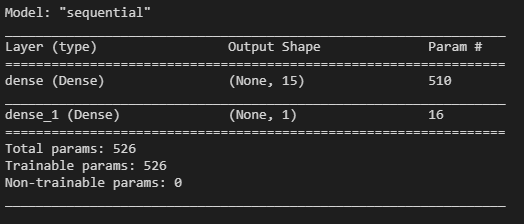
\includegraphics[width=0.7\linewidth]{Imagens/SumarioModeloNaoNormalziado}
	\caption{Sumário do Modelo MLP Não Normalizado}
	\label{fig:sumariomodelonaonormalziado}
\end{figure}

Como a figura \ref{fig:sumariomodelonaonormalziado} revela, nossa rede possui 1 camada escondida completamente conectada (densa) com 15 neurônios e a camada de saída com apenas 1 neurônio, cujo motivo fora explicado na seção \ref{sec:apresentacao}. Além disso, nota-se que o número de parâmetros treináveis é 526. Essa informação será importante quando variarmos o número de épocas de treinamento, que neste caso é 50, uma vez que possuir épocas demais pode significar um overfiting de nosso modelo, gerando perda de generalização. 

Para analisar a acurácia deste modelo, observemos as figuras abaixo.

\begin{figure}[H]
	\centering
	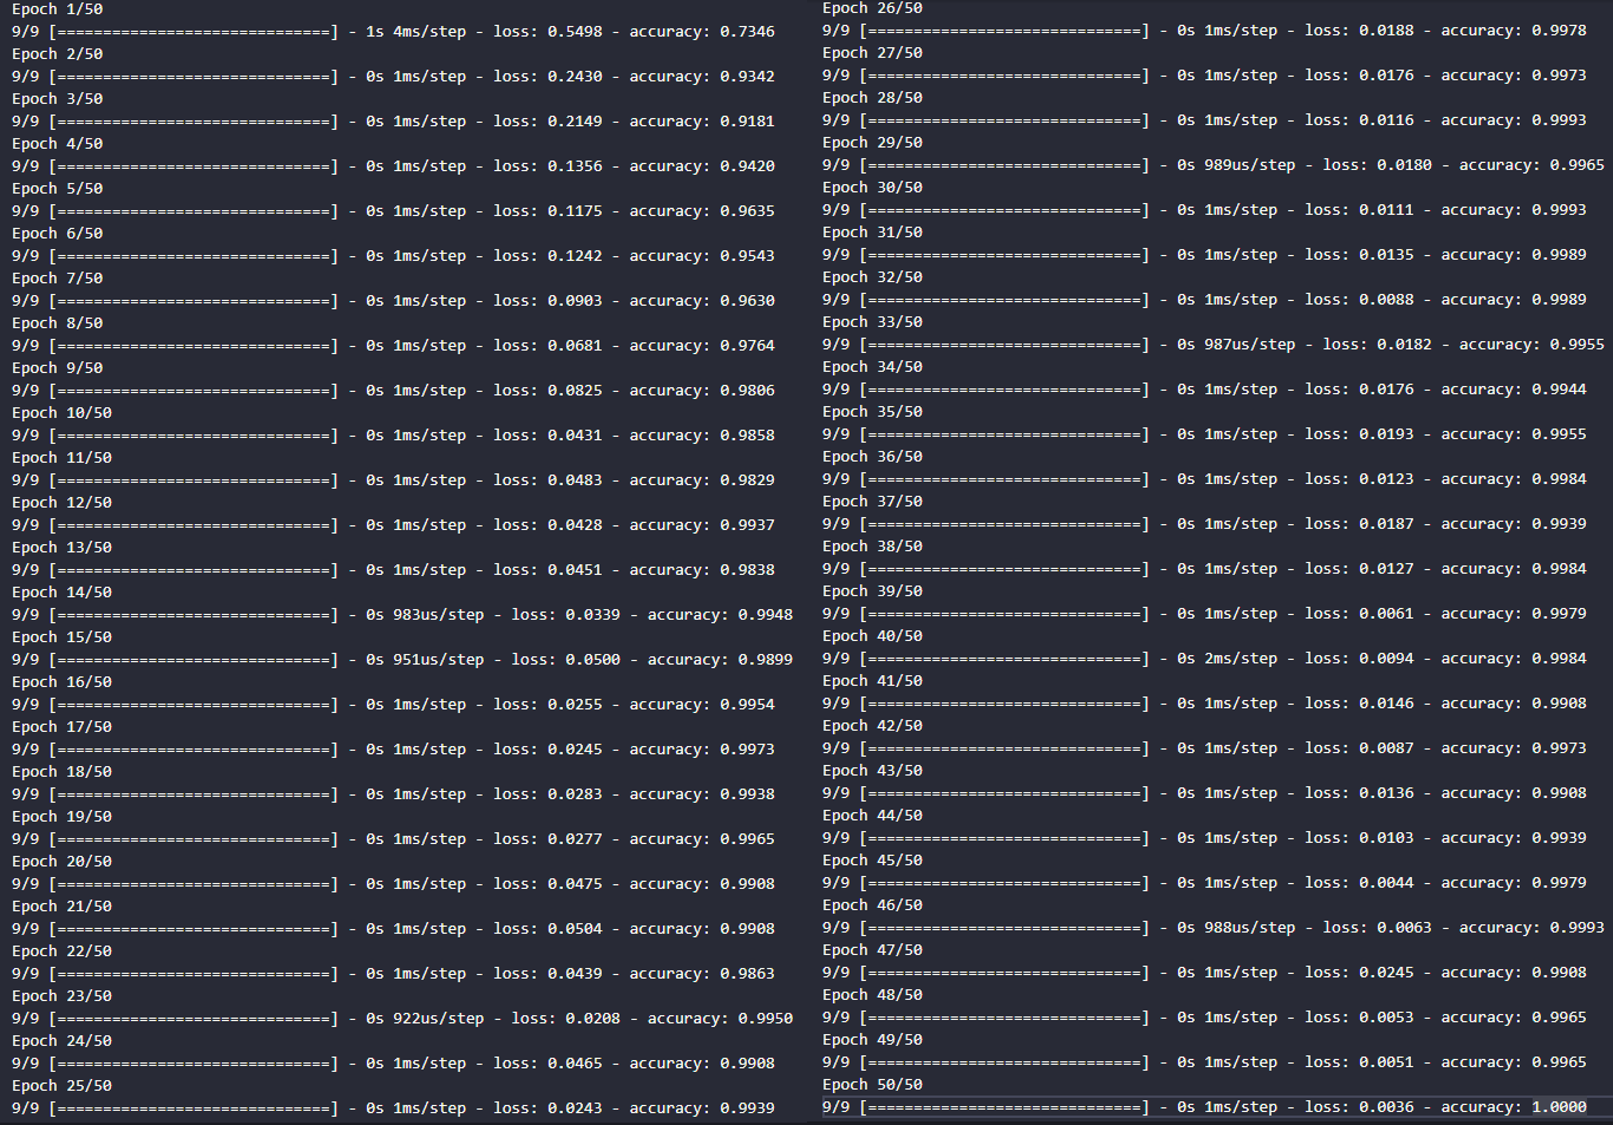
\includegraphics[width=1.1\linewidth]{Imagens/Fit_NaoNormalizado}
	\caption{Output do treinamento do modelo não normalizado}
	\label{fig:fitnaonormalizado}
\end{figure}

\begin{figure}[H]
	\centering
	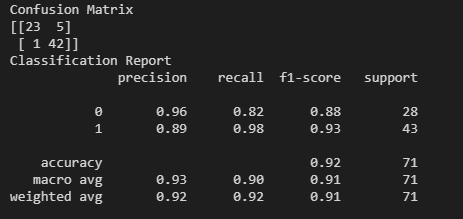
\includegraphics[width=0.7\linewidth]{Imagens/resultadoNaoNormalizado}
	\caption{Métricas do modelo não normalizado}
	\label{fig:resultadonaonormalizado}
\end{figure}

O modelo em questão apresentou acurácia de 92\%, o que, a priori, é bom, vide figura \ref{fig:resultadonaonormalizado}. Essa métrica indica que em 92\% dos casos apresentados na fase de validação a rede foi capaz de classificar corretamente o retorno como bom ou ruim. Podemos observar, também, que a evolução da acurácia do modelo na figura \ref{fig:fitnaonormalizado}. Percebe-se que, uma vez atingida a acurácia de 0.99 houve pouca flutuação nos valores dessa métrica, que na última época atingiu o valor de 1.00. Isso pode indicar que a quantidade de épocas não foi grande demais, pois, se fosse, veríamos uma queda maior na acurácia depois de certa época ou flutuações maiores em seu valor. Novamente, apenas quando testarmos outros valores de época poderemos confirmar se este foi (50) é um bom valor, mas, por hora, ele parece razoável. 

A precisão de nosso modelo foi de 0.96 para os casos zero, isto é, "bad" e de 0.89 para 1, "good". Isso nos mostra que a rede possui um grande desempenho em classificar corretamente os retornos ruins e um desempenho um pouco pior em classificar os retornos bons. Isso é curioso uma vez que a nossa base de treino foi composta de 182 entradas 1 e 98 entradas 0, o que mostra que nossos dados são razoavelmente desbalanceados. Uma solução possível para melhorar essa métrica é construir a base de treino de outra forma, garantindo maior equilíbrio entre os retornos bons e ruins. Na seção \ref{testelivre} faremos esse teste. Para a situação deste dataset, podemos argumentar que é melhor a rede classificar um retorno bom como ruim do que um retorno ruim como bom, uma vez que este segundo erro poderia causar a utilização de uma antena defeituosa, o que é mais prejudicial que não utilizar uma antena em bom funcionamento. Sendo assim, a rede indicar uma precisão maior para os retornos ruins é melhor do que o caso contrário, se ela apresentasse precisão menor para retornos ruins.

A métrica recall indica


\subsection{Agora normalize os dados de entrada e treine novamente o modelo MLP.	Avalie os resultados obtidos e comente o efeito da normalização no	treinamento da Rede Neural.}
	
\section{Mudança de configurações do modelo}

\subsection{Insira o conjunto de validação para o treinamento do modelo. Avalie o resultado obtido.}

\subsection{Modifique o tempo de treinamento (épocas) da Rede Neural. Escolha dois valores distintos (e.g. 1 e 1000 épocas) e avalie os resultados.}

\subsection{Modifique a taxa de aprendizado da Rede Neural. Escolha dois valores distintos (e.g. 0,001 e 0,1) e avalie os resultados.}

\subsection{Modifique a quantidade de neurônios na camada escondida da RedecNeural. Escolha dois valores distintos (e.g. 2 e 70 neurônios) e avalie os	resultados.}


\section{Teste Livre}\label{sec:testelivre}

\subsection{Faça novos testes para avaliar o desempenho da Rede Neural no	problema designado. Use a técnica K-Fold (com K = 10) para analisar o	resultado obtido.}

\subsection{Faça análises e novas implementações que você julgue importante para o seu trabalho. Não esqueça de explicar a motivação da análise realizada.}


\begin{thebibliography}{99} 
	
	\bibitem{Dataset} 
	UCI Machine Learning Repository,\\ \texttt{https://archive.ics.uci.edu/ml/datasets/Ionosphere}
	
	\bibitem{Paper1989} Sigillito, V. G., Wing, S. P., Hutton, L. V., \& Baker, K. B. (1989). \textit{Classification of radar returns from the ionosphere using neural networks.} Johns Hopkins APL Technical Digest, 10, 262-266.
	
	
	
	
	
	
\end{thebibliography}
\end{document}